\chapter{Higgs Phenomology}
\label{sec:pheno}

Dasu -
The pheno chapter need not start from the Dirac equation and build up. It should have crisp intro to Higgs phenomenology starting from that portion of the Lagrangian. You don’t need all the myriad details of SM like the quark mixing matrices, etc.

\section{Standard Model Symmetries}

\section{Electroweak Symmetry Breaking}

electroweak symmetry breaking is achieved via the Brout--Englert--Higgs
mechanism~\cite{Englert:1964et,Higgs:1964ia,Higgs:1964pj,Guralnik:1964eu,Higgs:1966ev,Kibble:1967sv},
leading, in its minimal version, to the prediction of the existence of one physical neutral scalar particle,
commonly known as the Higgs boson ($\PH$).


\section{Higgs Yukawa Couplings}
To establish the mass generation mechanism for fermions,
 it is necessary to probe the direct coupling of
the Higgs boson to such particles.
The most promising decay channel is $\Pgt^+\Pgt^-$,
because of the large event rate expected in the SM compared to the $\Pgm^+\Pgm^-$ decay channel ($\mathcal{B}(\PH\to\Pgt^+\Pgt^-)=6.3$\% for a mass of 125.09\GeV), and of the smaller contribution from background events
with respect to the $\bbbar$ decay channel.

\section{Higgs Production}

Feynman diagrams for the leading Higgs boson production processes
are shown in Figure~\ref{tab:higgs_feyn}.

The cross sections for the leading Higgs boson production processes
are shown in Figure~\ref{fig:higgs_production}. The values for the leading
process are approximately: $ggH \approx 48\pb$, VBF$ \approx 3.8\pb$, $\PW\PH \approx 1.4\pb$,
and $\PZ\PH \approx 0.88\pb$~\cite{deFlorian:2016spz}. The $\ttbar\PH$ process
which is found to be insignificant in the following analyses has a cross
section approximatly half the size of the next smallest one, $\PZ\PH$, where
$\ttbar\PH \approx 5.1\pb$.


\begin{figure*}[htbp]
\centering
     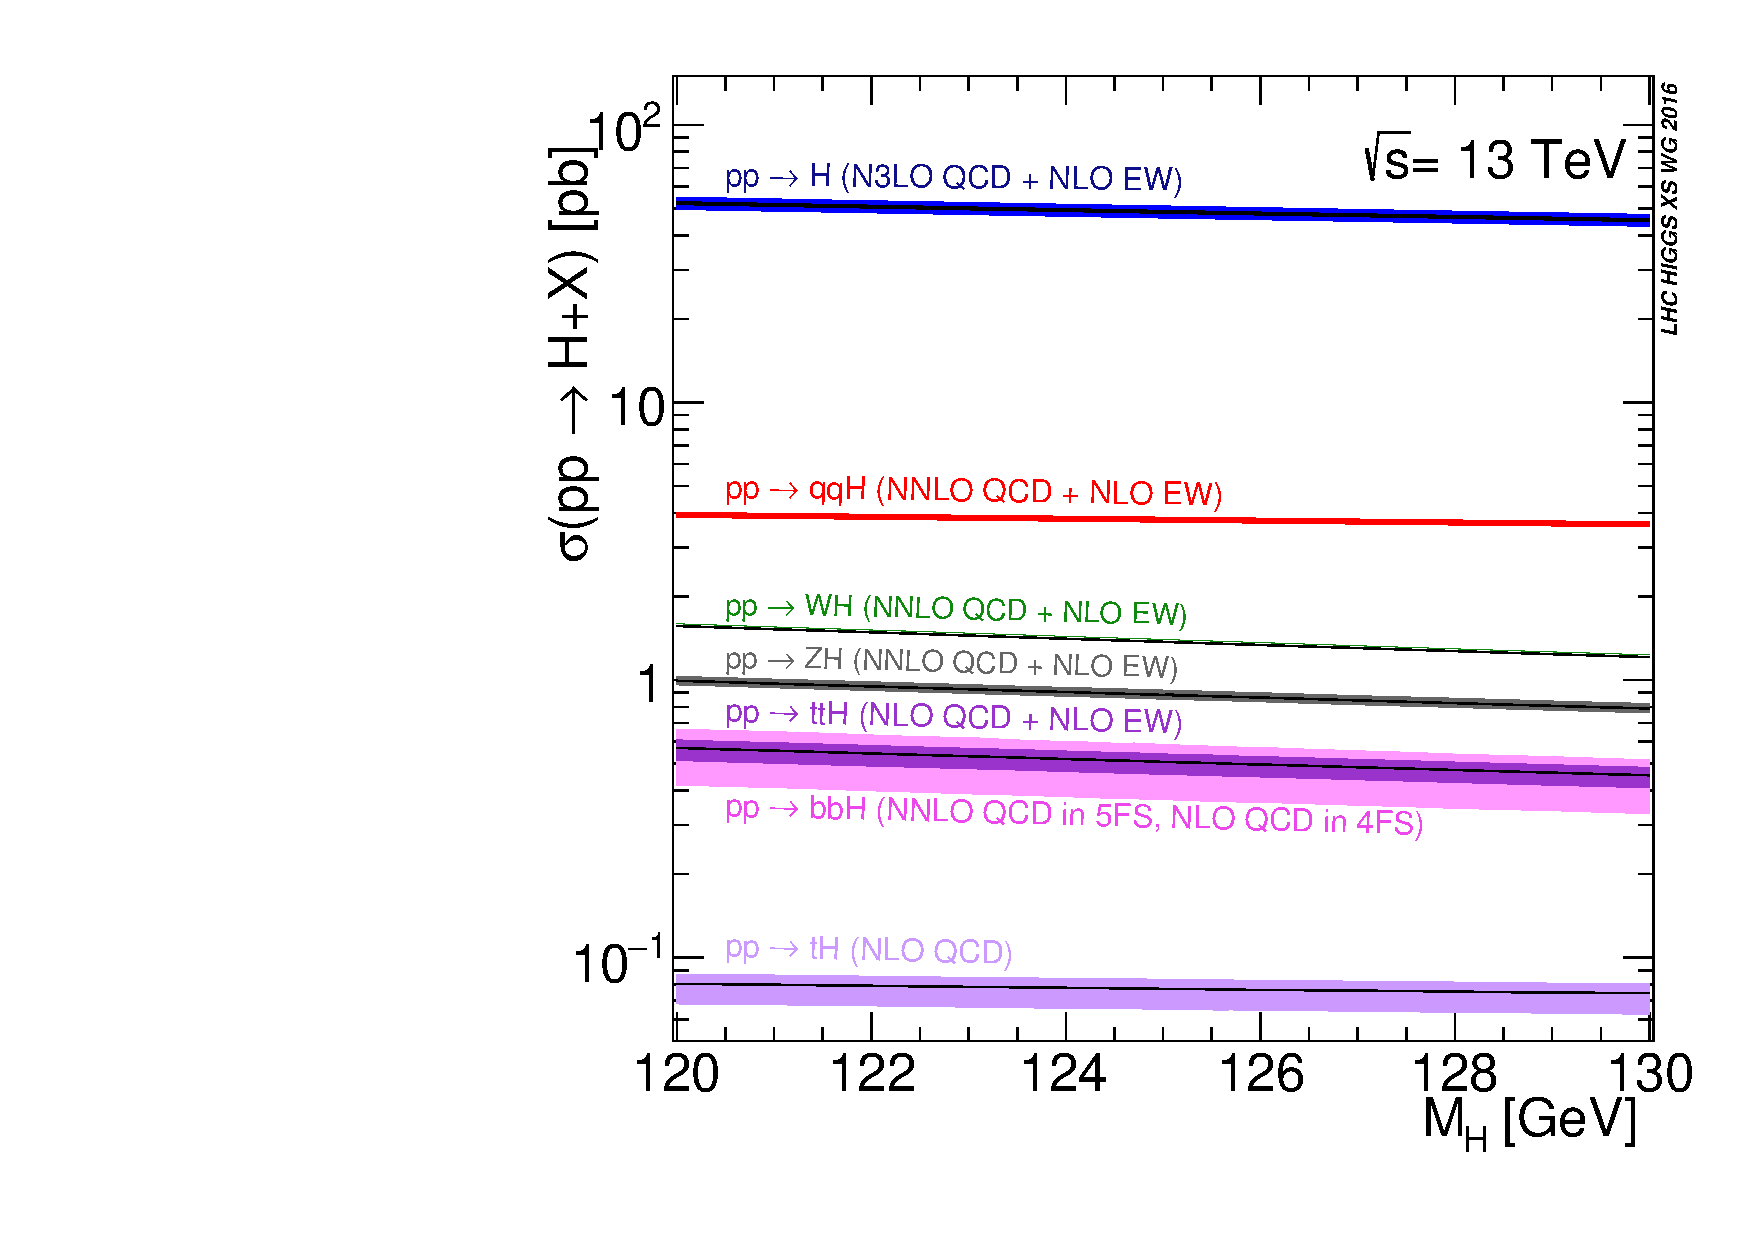
\includegraphics[width=0.65\textwidth]{phenomology_of_processes/plots/plot_13tev_H_sqrt.pdf}
     \caption{
The theorized Higgs boson production cross sections and their uncertainties,
as a function of the Higgs boson mass, are shown. The gluon fusion process ($ggH$)
is denoted as pp $\to$ H in the figure.
The CMS and ATLAS experiments have determined $\mH = 125.09\GeV$~\cite{Aad:2015zhl}.
     }
     \label{fig:higgs_production}
\end{figure*}


\subsection{Gluon Fusion}

\subsection{Vector Boson Fusion}

\subsection{Associated Production}

\section{Higgs Decays}

After a Higgs boson is produced, it will decay extremly rapidly. The theorized lifetime of a Higgs
boson particle is $1.6 \times 10^{-22}$ s~\cite{Dittmaier:2012vm} meaning that, when created
inside of the CMS detector, a Higgs boson will always decay
within the CMS detector . There are multiple possible decay
paths each with their own probability or branching ratio with the largest branching ratio
processes shown in Figure~\ref{fig:higgs_decay}. The $\htt$ process has a branching
ratio of approximately 6.3\% for $\mH = 125\GeV$.


\begin{figure*}[htbp]
\centering
     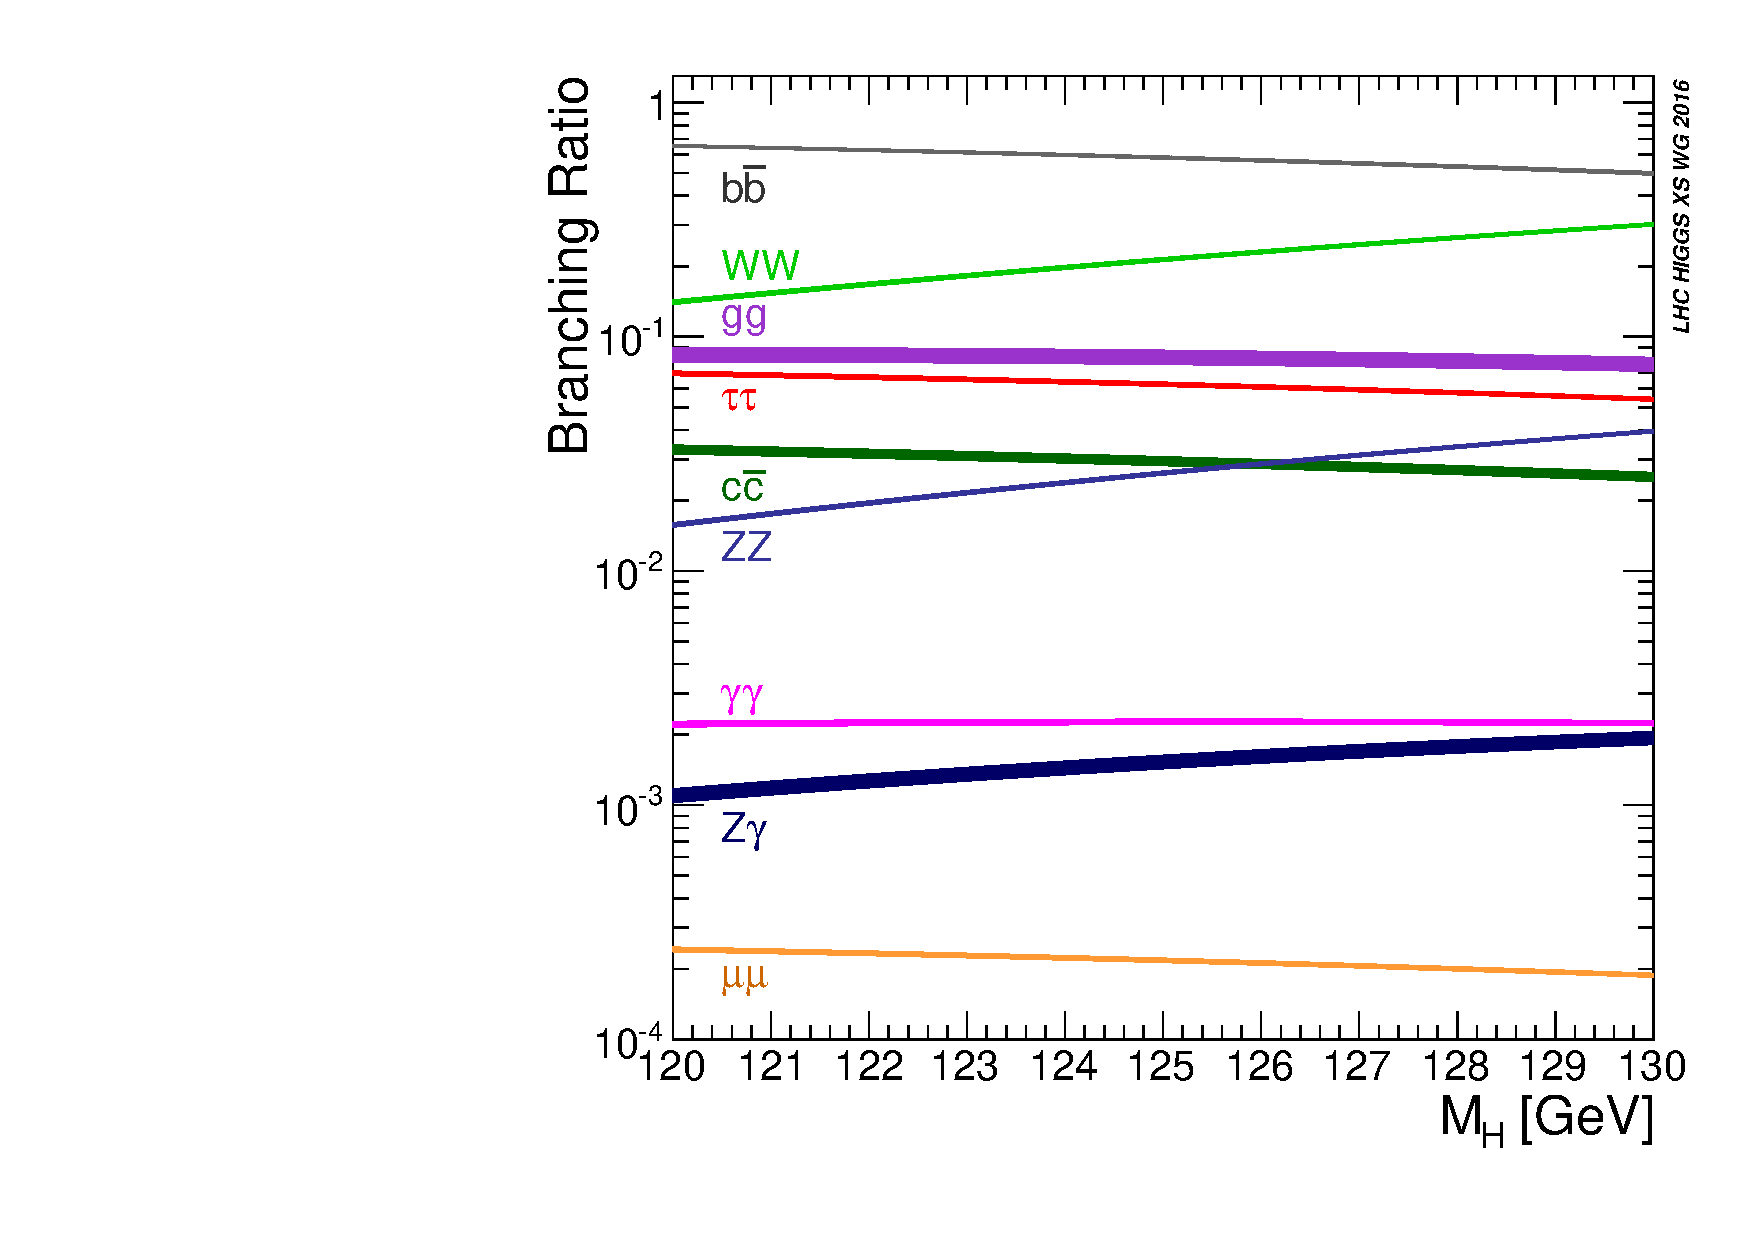
\includegraphics[width=0.65\textwidth]{phenomology_of_processes/plots/SMHiggsBR_YR4-square.pdf}
     \caption{
The different theorized Higgs boson decay process are shown as a 
as a function of the Higgs boson mass.
The CMS and ATLAS experiments have determined $\mH = 125.09\GeV$~\cite{Aad:2015zhl}.
     }
     \label{fig:higgs_decay}
\end{figure*}


\subsection{Higgs to $\tau\tau$ Decay Process}




The various production cross sections and branching fractions for the SM Higgs 
boson production, and their corresponding uncertainties are taken from 
References.~\cite{deFlorian:2016spz,Denner:2011mq,Ball:2011mu} and references therein.




%\subsection{QCD and Proton Structure}




